\documentclass[tikz,border=10pt]{standalone}
\usetikzlibrary{angles,quotes}
% Scale s = 0.019324 cm/px, origin at B, y flipped about px y=301
\begin{document}
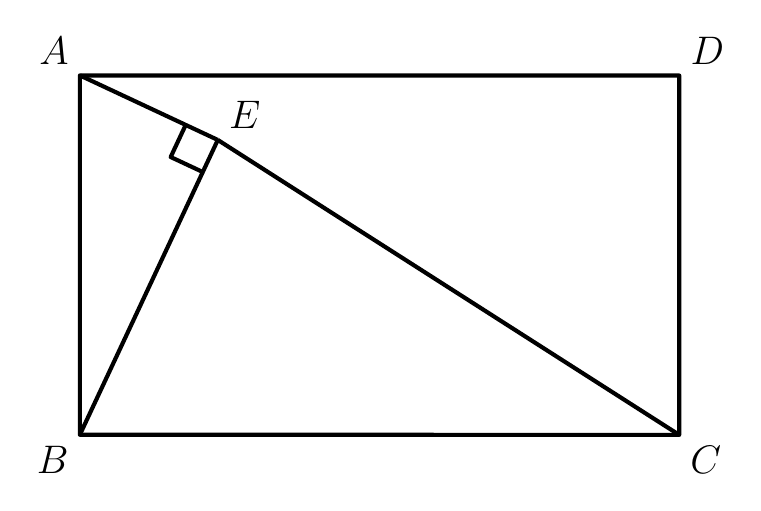
\begin{tikzpicture}[line width=1.5pt, line join=round,
  lbl/.style={font=\fontsize{15.5}{18.6}\selectfont}]
  % Vertices (measured; A-E-C is a shallow bend, E kept off line AC)
  \coordinate (A) at (0.0027793718297619563,4.56357855568368);
  \coordinate (B) at (0.0018666292817877128,0.00014681040460473582);
  \coordinate (C) at (7.613523017423969,-0.0013756146110002199);
  \coordinate (D) at (7.614435759971943,4.562056130668075);
  \coordinate (E) at (1.7537588895852747,3.744292120093804);
  % Rectangle edges
  \draw (A) -- (D) -- (C) -- (B) -- cycle;
  % Interior edges: polyline A-E-C and E-B
  \draw (C) -- (E);
  \draw (E) -- (B);
  \draw (A) -- (E);
  % Single right-angle mark at E between arms EA and EB
  \pic[draw, angle radius=0.45cm, angle eccentricity=1.0] {right angle=A--E--B};
  % Labels outside the figure
  \node[above left, lbl] at (A) {$A$};
  \node[above right, lbl] at (D) {$D$};
  \node[below left, lbl] at (B) {$B$};
  \node[below right, lbl] at (C) {$C$};
  \node[above right, lbl] at (E) {$E$};
\end{tikzpicture}
\end{document}